\documentclass[border=6pt]{standalone}
% Shared preamble for web figures.  Each figure is a standalone .tex that
% \input's this file; scripts/make-figures.sh turns it into an SVG.
% Handouts pull the same file with \fig{Unit_X/<name>}.
\usepackage[T1]{fontenc}
\usepackage{helvet}
\renewcommand{\familydefault}{\sfdefault}
\renewcommand{\ttdefault}{pcr}  % Courier: a real Type 1 typewriter font
\usepackage{amsmath}
\usepackage{tikz}
\usetikzlibrary{arrows.meta,positioning,calc,shapes.symbols,shapes.geometric}

% Who makes the rules is the point of most diagrams in this book, so the
% colors mean the same thing everywhere: blue is a person, orange is the
% computer, green is an answer, pink is the human brain.
\definecolor{person}{HTML}{2C6FAE}
\definecolor{machine}{HTML}{D35400}
\definecolor{result}{HTML}{1E8449}
\definecolor{brainpink}{HTML}{C2185B}
\definecolor{ink}{HTML}{2C3E50}

\tikzset{
  doodle/.style={line width=1.5pt, line cap=round, line join=round, draw=ink},
  box/.style={draw, rounded corners=5pt, line width=1.1pt, align=center,
              inner sep=7pt, minimum height=1.0cm, font=\small},
  personbox/.style={box, draw=person, fill=person!10},
  machinebox/.style={box, draw=machine, fill=machine!10},
  resultbox/.style={box, draw=result, fill=result!10},
  plainbox/.style={box, draw=ink!70, fill=ink!4},
  flow/.style={-{Stealth[length=8pt]}, line width=1.4pt, draw=ink},
}

% A person (blue) and a robot head (orange) as small icons.
% \personicon{x}{y}{scale}   \roboticon{x}{y}{scale}
\newcommand{\personicon}[3]{%
  \begin{scope}[shift={(#1,#2)}, scale=#3]
    \fill[person] (0,0.62) circle (0.28);
    \fill[person, rounded corners=6pt] (-0.42,-0.55) rectangle (0.42,0.28);
  \end{scope}}
\newcommand{\roboticon}[3]{%
  \begin{scope}[shift={(#1,#2)}, scale=#3]
    \draw[machine, line width=1.2pt] (0,0.5) -- (0,0.72);
    \fill[machine] (0,0.78) circle (0.08);
    \draw[machine, line width=1.4pt, fill=machine!12, rounded corners=4pt] (-0.5,-0.45) rectangle (0.5,0.5);
    \fill[ink] (-0.2,0.12) circle (0.08);
    \fill[ink] (0.2,0.12) circle (0.08);
    \draw[ink, line width=1pt] (-0.22,-0.22) -- (0.22,-0.22);
  \end{scope}}

\begin{document}
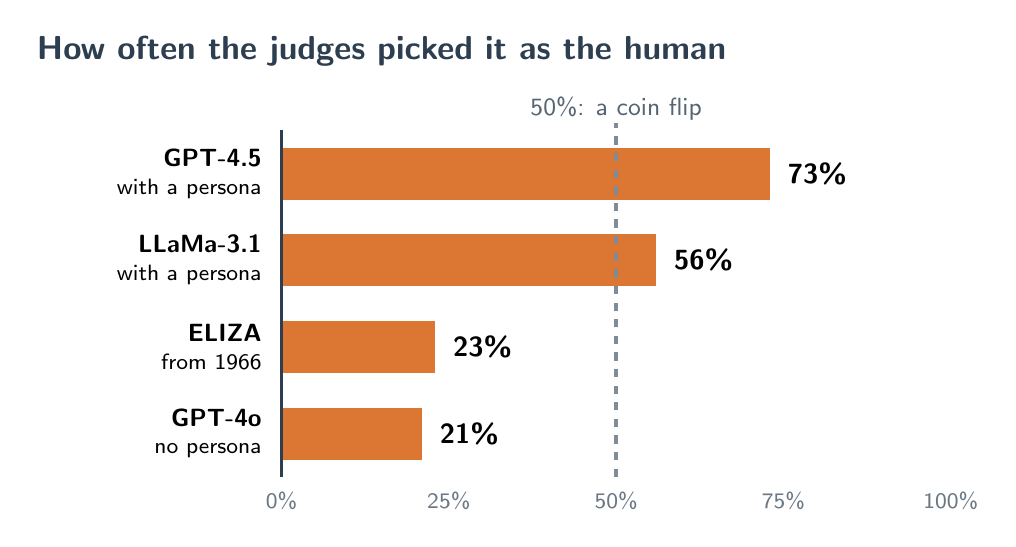
\begin{tikzpicture}[x=0.085cm, y=1cm]
% Jones & Bergen (2025), three-party Turing test: how often each system was
% picked as the human.  Data from the paper's abstract (arXiv 2503.23674).
\node[anchor=west, font=\large\bfseries, text=ink] at (-38,5.15) {How often the judges picked it as the human};
\foreach \v/\name/\sub/\y in {73/GPT-4.5/with a persona/3.6, 56/LLaMa-3.1/with a persona/2.5, 23/ELIZA/from 1966/1.4, 21/GPT-4o/no persona/0.3} {
  \fill[machine!80] (0,\y-0.33) rectangle (\v,\y+0.33);
  \node[anchor=west, font=\bfseries] at (\v+1.2,\y) {\v\%};
  \node[anchor=east, align=right, font=\small] at (-1.5,\y) {\textbf{\name}\\[-1pt]{\footnotesize\sub}};
}
\draw[ink, line width=0.8pt] (0,-0.25) -- (0,4.15);
\draw[ink!60, dashed, line width=1.2pt] (50,-0.25) -- (50,4.25);
\node[anchor=south, font=\small, text=ink!80, align=center] at (50,4.15) {50\%: a coin flip};
\foreach \t in {0,25,50,75,100} \node[font=\footnotesize, text=ink!70] at (\t,-0.55) {\t\%};
\end{tikzpicture}
\end{document}
